\chapter{Introduction to FPGA Architectures for Machine Learning and Hardware Acceleration}

\section[Introduction]{\textbf{Introduction}}
%% BEGIN CONTENT HERE
The exponential growth of machine learning (ML) across domains such as healthcare, finance, autonomous systems, and natural language processing has driven a parallel need for hardware platforms capable of executing ML models with high throughput, low latency, and energy efficiency. While data centers have traditionally handled most of this computation using CPUs and GPUs, there is now a critical push to bring ML closer to the source of data — on edge and embedded devices — where constraints on power, size, and compute capability are far more stringent.

Conventional general-purpose processors (CPUs) are not well-suited for ML inference tasks due to limited parallelism and sequential instruction execution. Graphics processing units (GPUs), though highly parallel, consume considerable power and rely heavily on memory bandwidth, which can become a bottleneck for real-time or streaming applications. As a response to these limitations, field-programmable gate arrays (FPGAs) have garnered attention due to their reconfigurability, high-performance-per-watt ratio, and ability to implement custom parallel datapaths for specific ML operations.

Despite these advantages, FPGA design for ML is far from straightforward. Several challenges exist, such as selecting the most suitable internal architecture (e.g., use of carry chains vs. DSP blocks), managing memory hierarchies, balancing performance with resource usage, and designing application-specific accelerators that leverage the unique strengths of the FPGA fabric.

This project, titled "Design of Efficient ML Hardware: FPGA Architectural Optimization and Domain-Specific Hardware", is a comprehensive attempt to tackle these challenges from two complementary perspectives:
\begin{enumerate}
	\item \textbf{Architectural Exploration Using the VTR Toolchain:} This component investigates and compares different FPGA fabric architectures — particularly carry chain-based versus DSP block-centric designs — for their efficiency in handling ML-centric benchmarks. The study focuses on low-precision arithmetic, approximate computing, and non-standard number representations commonly used in neural networks and digital signal processing. Benchmark circuits such as adder trees and FIR filters are refactored to utilize carry chains effectively, and performance metrics such as delay, area, and power are evaluated.
	\item \textbf{Design of a Domain-Specific Accelerator – Manojavam:} This custom-built hardware accelerator targets Principal Component Analysis (PCA), a widely used dimensionality reduction technique in ML. The design includes an array of TPU-style 4×4 systolic arrays for matrix multiplication and a novel Jacobian Unit that uses the Jacobi method to perform eigendecomposition. The architecture incorporates efficient memory access patterns through block streaming and cache hierarchies and is implemented entirely in RTL. Manojavam was synthesized and tested on an FPGA (Xilinx Artix-7), and also realized through ASIC flow using OpenLane.
\end{enumerate}

This dual-focus effort is especially relevant in the current era where ML model optimization must go hand-in-hand with hardware optimization. The ability to fine-tune the architecture — either by modifying the FPGA fabric or by building domain-specific RTL pipelines — is critical for improving performance-per-watt and ensuring scalability in edge ML applications.

In essence, this project bridges two essential layers of ML acceleration — architectural suitability and domain-specific hardware design — making it not only a technically enriching exploration but also a contribution toward the future of ML compute platforms.

\begin{comment}
	content..
The title of the project can be introduced in this section. This section should neatly elaborate the context of the project, the relevance of the area chosen and the title. You can bring a brief history and arrive at the title of the project. Use appropriate number of paragraphs within this section. 

You are allowed to use figures or diagrams which can help in introducing the topic acknowledging the source. For example , if you are introducing a particular topic, an appropriate figure can be used. The figure should be referenced in the text as Figure. \ref{fig:universe} 
\begin{figure}[htb]
\centering
	
\includegraphics[scale=1]{Figures/universe}	
	\caption{Sample picture of universe }
	\label{fig:universe}
\end{figure}

These guidelines are provided to formally expose you to the various ethical and technical issues involved in writing up your work and the format you are required to adhere to while submitting your project report.
\end{comment}

\section[Motivation]{\textbf{Motivation}}
%% BEGIN CONTENT HERE
The motivation behind choosing this project stems from two persistent and interrelated challenges in the field of machine learning hardware: the need for energy-efficient, real-time ML execution platforms suitable for edge devices, and the growing importance of performing architectural exploration of FPGA platforms using established frameworks such as the widely adopted VTR toolchain, particularly in the context of ML-centric workloads.

As ML becomes increasingly embedded into devices like drones, sensors, wearables, and autonomous systems, the demand for compact, low-power hardware accelerators has intensified. General-purpose processors fall short due to their serial execution model, while GPUs — though powerful — are often unsuitable for power-sensitive environments. This made the case for exploring FPGAs, which offer flexibility and energy efficiency. However, the choice of FPGA internal architecture significantly impacts ML performance. The first part of the project involved evaluating existing FPGA architectures using the VTR toolchain. Architectures were assessed using adder tree and FIR filter benchmarks, which are representative of machine learning workloads due to their reliance on fundamental operations like addition and multiplication.

Simultaneously, in academic and applied research, Principal Component Analysis (PCA) remains a cornerstone of dimensionality reduction in ML and signal processing. Yet, very few hardware implementations efficiently support PCA operations like covariance matrix computation and eigendecomposition. This motivated the second part of the project — designing Manojavam, a domain-specific accelerator that performs PCA using custom RTL logic.

The idea of combining architectural benchmarking with the design of a complete hardware accelerator emerged as a powerful way to bridge theory and application. It allowed for deep exploration of both low-level FPGA features and high-level ML operations, and aligned well with current trends in edge AI and domain-specific hardware design.

\begin{comment}
Brief the motivation of selecting your project title. You can elaborate the challenges in the specific area, relevance and importance of the chosen topic. 
\end{comment}

\section[Problem statement]{\textbf{Problem statement}}
%% BEGIN CONTENT HERE
General-purpose processors are inherently inefficient for machine learning (ML) workloads due to their limited parallelism, sequential instruction execution, and high power consumption, while GPUs, though better suited for compute-intensive tasks, suffer from excessive energy usage and memory bandwidth constraints. Although FPGAs offer a promising balance of configurability, parallelism, and energy efficiency, current FPGA architectures are not optimized for ML tasks, particularly those involving low-precision arithmetic or approximate computing. At the same time, domain-specific accelerators capable of performing foundational ML algorithms like Principal Component Analysis (PCA) in an efficient and scalable manner are largely absent in RTL-level research and development. This project aims to address these challenges by conducting an architectural exploration of FPGA fabrics for ML workloads and designing a custom PCA accelerator, Manojavam, capable of efficient covariance matrix computation and eigendecomposition using systolic arrays and RTL-based optimization.

\begin{comment}
	Define the problem statement in this section, in one paragraph.
\end{comment}

\section[Objectives]{\textbf{Objectives}}
%% BEGIN TEXT HERE
The objectives of the project are-
\begin{enumerate}
	\item To explore and evaluate FPGA architectural features, specifically carry chain-based designs versus DSP block-based architectures, for their suitability in machine learning workloads using the VTR toolchain.
	\item To design and implement a domain-specific hardware accelerator named Manojavam for Principal Component Analysis (PCA), featuring matrix multiplication using systolic arrays and eigendecomposition using a custom Jacobian Unit.
	\item To synthesize, simulate, and validate the proposed accelerator on both FPGA and ASIC flows, and compare its performance with conventional CPU/GPU implementations as well as existing state-of-the-art PCA accelerators.
\end{enumerate}

\begin{comment}
The objectives of the project are
\begin{enumerate}
\item To design a pipelined ADC for audio frequency range
\item List all the objectives in the above format , starting with "To"
\item Limit the number of objectives to a maximum of three
\end{enumerate}
\end{comment}

\section[Literature Review]{\textbf{Literature Review}}
%% BEGIN CONTENT HERE
\subsection{Related Work on FPGA Architectural Exploration for ML Workloads}
Over the past three decades, the architecture of Field-Programmable Gate Arrays (FPGAs) has undergone extensive evolution, driven by the increasing complexity of target applications and advances in process technologies. A core objective of FPGA architecture research has been to balance flexibility with performance, area efficiency, and power consumption.

Initial FPGA designs employed basic logic elements (BLEs) consisting of small look-up tables (LUTs) and flip-flops. These BLEs were clustered into larger logic blocks with local interconnect to enhance packing efficiency and reduce inter-block routing delay. Ahmed and Rose\cite{ahmed2000effect} empirically studied the area-delay trade-offs of different LUT sizes and BLE clusterings, concluding that 4–6 input LUTs and cluster sizes of 3–10 BLEs provide an optimal area-delay product. Fracturable LUTs were introduced in Altera’s Stratix II\cite{stratix2007stratix} and Xilinx’s Virtex-5\cite{xilinxvirtex} to mitigate underutilization in large LUTs. These allowed a single 6-LUT to be decomposed into two 5-LUTs, improving logic density and enabling more effective packing of smaller functions.

Arithmetic operations—especially additions and multiplications—are central to many FPGA applications, from DSP to machine learning. Initially, such operations were implemented using LUTs, but this approach suffered from excessive logic utilization and long critical paths. To address this, modern FPGAs integrate hardened carry chains within their logic elements. Murray et al\cite{boutros2019math} found that 22\% of the logic elements in typical FPGA workloads implement arithmetic, justifying the need for specialized support. Their study shows that hardening carry chains improves performance by 75\% for arithmetic microbenchmarks and 15\% for general workloads.

The latest Intel Agilex devices\cite{intel_agilex_2020} and Xilinx Versal architecture\cite{xilinx_versal_trm_2021} further advance this trend by implementing carry-skip and carry-lookahead adders, respectively. The Agilex architecture hardens 2-bit carry-skip adders per logic element, enabling dense and high-speed arithmetic, while Versal enables 1-bit per logic element with advanced carry logic. Stratix devices also use fracturable 6-LUTs that support 2-bit arithmetic per adaptive logic module (ALM), achieving both compact area and high arithmetic throughput.

Proposals to enhance arithmetic density include logic elements with 4-bit carry chains arranged in single or dual configurations\cite{boutros2019math}\cite{boutros2021fpga}. These studies demonstrated that dual-chain configurations improve multiply-accumulate (MAC) operation density by up to 17\% and reduce area by 8\%, showing promise for arithmetic-intensive ML and DSP workloads.

A critical aspect of FPGA architecture research is evaluating trade-offs across area, timing, and power. The typical methodology involves defining an architecture model, selecting benchmark circuits, and utilizing a CAD toolchain to simulate implementation results\cite{boutros2021fpga}. The Verilog-to-Routing (VTR) tool\cite{rose2012vtr} is a widely used open-source CAD framework for this purpose. It allows researchers to model custom FPGA architectures through descriptive XML files, map benchmark designs, perform placement and routing, and obtain post-routing metrics. This methodology underpins much of the academic work in architecture exploration and was adopted in the present study for fair evaluation of different carry chain designs.

Benchmarking traditionally relied on the MCNC suite\cite{yang1991logic}, which includes small logic-centric designs. However, these are no longer representative of modern FPGA applications. The Titan benchmark suite\cite{rose2012vtr}, derived from industrial designs, provides larger and more realistic circuits and has become a standard in architecture evaluation. Other works have emphasized the need for emerging benchmark suites that better reflect ML and signal-processing-heavy workloads.

Modern commercial FPGAs have embraced increasing heterogeneity, incorporating DSP blocks, embedded memories, and even hardened interconnect pipelining. For example, Intel’s Stratix 10 integrates optional pipeline registers within routing drivers using configurable pulse latches\cite{intel_stratix10_2019}, while Xilinx Versal includes input-side block registers to reduce long interconnect delay\cite{xilinx_versal_trm_2021}. These additions aim to mitigate timing bottlenecks associated with deeper pipelining in high-performance workloads.

Additionally, attempts to repurpose the logic fabric for low-precision ML tasks, such as implementing 8-bit MACs using LUTs and carry chains\cite{boutros2021fpga}, have driven research into logic elements that better support partial product reduction and carry-propagation efficiency. Carry chains have proven useful in implementing tree-based multipliers and accumulators, underscoring their utility beyond addition.

\subsection{Related Work on PCA and SVD Accelerators}
There have been attempts to overcome computational challenges associated with Principal Component Analysis (PCA) and Singular Value Decomposition (SVD). As PCA and SVD are inherently related to each other, the below sections highlight the state of art approaches to accelerate both PCA and SVD workloads on high performance computing hardware. 

%%% All PCA Architecture Surveys
%\subsection{Principal Component Analysis (PCA) : Approaches and Architectures}

In \cite{pca_architecture-1}, the authors implement a full fledged accelerator for Principal Component Analysis, where the architecture solves both the learning and mapping phases. They implement eigenvalue decomposition using QR factorization with Givens CORDIC rotation on the computed covariance matrix. The accelerator works at an operational frequency of 183 MHz, and consumes 56\% of LUTs, 19\% of memory and 88\% of the DSP blocks, on a Xilinx Virtex-7 FPGA. However, the design does not scale well for large matrices and operates better than an Nvidia GPU and Intel processors for small matrices, with a maximum tested dimension of 16×30. The authors employ a parallel vector based matrix multiplication approach. 

A reconfigurable PCA accelerator was proposed in \cite{pca_architecture-2}, where the accelerator was employed to preprocess data from satellites to the ground in low bandwidth scenarios, saving them cost. The authors implemented an EVD engine, and used a DMA module with prefetching to hide latencies associated with memory bottlenecks. The architecture employs 67\% of the available FPGA resources, and shows a performance improvement of 10x and 12x on the AVIRIS Cuprite and Jasper datasets respectively. However, the chip does not accelerate matrix multiplication, and the authors claim that it consumes too much overhead, and works faster on software. Moreover, the key microarchitectural details about the Jacobi algorithm are not revealed. 

A full-fledged PCA accelerator was proposed in \cite{pca_architecture-3}, implementing both learning and mapping phases, designed entirely using High-Level Synthesis (HLS). The primary application of the accelerator is hyperspectral imaging, where it computes the covariance matrix of the input dataset using a Covariance Unit and performs Eigenanalysis through an SVD unit. However, the paper does not disclose specific microarchitectural details of these units. The design was implemented on two FPGA platforms: the Zynq-7000 XC7Z020CLG484-1 and the Virtex-7 XC7VX690TFFG1761-2, with reported power consumption of 2.376W and 9.786W, respectively. A notable drawback of the design is its reliance on HLS, which, while simplifying hardware development, abstracts away low-level optimizations that could improve efficiency and performance. 

An outlier detection scheme for Network Intrusion Detection Systems (NIDS) is proposed in \cite{pca_architecture-4}, leveraging Principal Component Analysis for anomaly detection after an initial Feature Extraction Module (FEM) processes the network traffic. The PCA framework follows a two phase approach : an offline PCA phase, where the principal components are obtained from a training dataset, and the online PCA phase, where the incoming data is projected onto these principal components to detect outliers in real time. The authors note that while PCA significantly reduces the computational complexity, eigenvector calculations and sorting remain sequential and difficult to parallelize, making them less suited for FPGA based acceleration. However, the principal component score calculations, which involve matrix to vector computations, are efficiently parallelized in hardware. 

A dynamic on-the-fly reconfigurable PCA accelerator was proposed in \cite{pca_architecture-5}, where the accelerator dynamically reconfigures itself during different stages of the PCA algorithm. The implementation was developed on the ML605 FPGA board, which is based on 40 nm CMOS technology and features a Xilinx Virtex-6 (XC6VLX240T-FF1156) FPGA, MicroBlaze soft processors, 2MB of on-chip BRAM, and 512MB of DDR3-SDRAM for large-scale data storage. The design was implemented using a mix of Verilog and VHDL and operates at a maximum clock frequency of 100 MHz. The authors employed a Covariance Unit to compute the covariance matrix efficiently and used QR factorization for Eigenvalue Decomposition (EVD). However, the paper does not provide microarchitectural details of these units. While dynamic reconfiguration led to a 71\% area savings, it introduced significant reconfiguration overheads in the order of milliseconds, which could degrade overall performance. Additionally, the authors note that while the cyclic Jacobi method is effective for small matrices, alternative methods such as QR or Householder decomposition may be better suited for larger matrices.

%%% All SVD Architecture Surveys
%\subsection{Singular Value Decomposition (SVD) : Approaches and Architectures}

The work in \cite{svd_architecture-1} proposes an FPGA accelerator for Singular Value Decomposition employing fixed point arithmetic, using the Hestenes-Jacobi algorithm and CORDIC. The accelerator works at an operational frequency of 250 MHz on a Xilinx Kintex-7 XC7K325T FPGA. It achieves a speedup between 8.5× and 15.3× over MATLAB and between 2.1× and 6.3× over GPU implementations. However, the design is not scalable to very large matrices due to block RAM limitations, and the authors suggest that an array of FPGAs may be needed for handling larger matrices beyond 128×128. 

An FPGA based accelerator for both Singular Value Decomposition and Eigenvalue Decomposition is proposed in \cite{svd_architecture-2}, where the accelerator is optimized for real time performance. The accelerator is based on the Jacobi algorithm, employing the Brent-Luk systolic array to efficiently compute SVD, and using CORDIC based algorithm for EVD. The design, when dumped on the Xilinx Virtex-5 FPGA, operates at a frequency of 130 MHz, and shows a performance improvement of 4x compared to a 2.53 GHz Intel processor, and an improvement of 2x for EVD when compared to the previous FPGA based designs. The hardware utilization for an 8×8 matrix reaches 98\%, but while this demonstrates high efficiency, the increasing resource demand for larger matrices may impact scalability. 

The work in \cite{svd_architecture-3} proposes an SVD engine, designed on 90nm CMOS technology, wth an operational frequency of 101.2 MHz and a power of 125 mW, for very high throughput MIMO-OFDM systems. The authors implemented an adaptive SVD engine, which would dynamically modify the output eigenvectors and values with changes in inputs. An Orthogonal Reconstruction (OR) scheme is also implemented to correct errors due to fixed point arithmetic, ensuring very high accuracy. However, the SVD engine primarily relies on a sequential execution model, particularly in Jacobi-based updates and CORDIC-based rotations, which may limit scalability for larger matrices beyond 4×4. 

The work in \cite{svd_architecture-4} compares and contrasts the execution of the Jacobi algorithm on the CPU, GPU, and FPGA, revealing that the GPU suffers from performance degradation due to unstructured global memory access patterns. To address this, the paper proposes three enhanced memory access patterns—Modified Access (MA), Symmetric Access (SA), and Maximum Coalesced Access (MCA)—which significantly improve GPU performance. The study highlights the critical role of memory access optimization in accelerating the Jacobi algorithm, particularly for GPU implementations, while also confirming that FPGA outperforms both GPU and CPU in overall efficiency for eigenanalysis. 

The work in \cite{svd_architecture-5} proposes a parallel fast-converging Jacobi algorithm designed for larger matrices, improving upon traditional Jacobi-based methods. Instead of processing elements in a fixed order, the algorithm selects N/2 of the largest off-diagonal elements in each iteration while maintaining row-column exclusivity. This reduces the number of Jacobi sweeps required and accelerates convergence. The design employs CORDIC-based rotations for efficient computation of trigonometric functions and is implemented on the Xilinx Virtex-6 XCVLX365T FPGA. Although the engine introduces an optimized Jacobi approach, it does not include a dedicated matrix multiplication accelerator to enhance intermediate transformations within the algorithm. As a result, row and column updates rely solely on DSP-based multipliers, which may introduce computational bottlenecks for larger matrices. Integrating a matrix multiplication accelerator (such as a systolic array or TPU-like cores) could further improve the throughput and scalability of the SVD core, especially for matrices beyond 32×32. 

A Hestenes-Jacobi processor for SVD was developed in \cite{svd_architecture-6}, which computed SVD for arbitrary size matrices in IEEE-754 double precision floating point format. The architecture comprised three dedicated units : the Hestenes Preprocessor, Jacobi Rotation unit and the Update unit. The authors do not employ a systolic array for matrix multiplication, noting that traditional systolic architectures are optimized for square matrices. However, the paper neither explores nor considers alternative approaches such as block-streaming systolic architectures, which could potentially improve efficiency in rectangular matrix multiplications. The design was dumped on a Xilinx Virtex-5 XC5VLX330 FPGA, operating on 150 MHz, consuming 89\% LUTs, 91\% BRAMs and 53\% DSPs. Matrices of dimension in the order of 1024 were tested successfully. However, they employ Xilinx Coregen IPs in their design, consuming 9, 14, 57 and 57 clock cycles for multiplier, adder-subtractor, divider and square root blocks respectively. 


\begin{comment}
A literature review is a text of a scholarly paper, which includes the current knowledge including substantive findings, as well as theoretical and methodological contributions to a particular topic. Literature reviews are secondary sources, and do not report new or original experimental work. Most often associated with academic-oriented literature, such reviews are found in academic journals, and are not to be confused with book reviews that may also appear in the same publication. Literature reviews are a basis for research in nearly every academic field . A narrow-scope literature review may be included as part of a peer-reviewed journal article presenting new research, serving to situate the current study within the body of the relevant literature and to provide context for the reader. In such a case, the review usually precedes the methodology and results sections of the work.

\subsection{Sample}
The main types of literature reviews are: evaluative, exploratory, and instrumental. A fourth type, the systematic review, is often classified separately, but is essentially a literature review focused on a research question, trying to identify, appraise, select and synthesize all high-quality research evidence and arguments relevant to that question. A meta-analysis is typically a systematic review using statistical methods to effectively combine the data used on all selected studies to produce a more reliable result.
\subsubsection[Review types]{\textbf{Review types}}

The main types of literature reviews are: evaluative, exploratory, and instrumental. A fourth type, the systematic review, is often classified separately, but is essentially a literature review focused on a research question, trying to identify, appraise, select and synthesize all high-quality research evidence and arguments relevant to that question. A meta-analysis is typically a systematic review using statistical methods to effectively combine the data used on all selected studies to produce a more reliable result.


\subsubsection[Process and product]{\textbf{Process and product}}

Distinguish between the process of reviewing the literature and a finished work or product known as a literature review. The process of reviewing the literature is often ongoing and informs many aspects of the empirical research project. All of the latest literature should inform a research project. Scholars need to be scanning the literature long after a formal literature review product appears to be completed.

\subsubsection{\textbf{Page limitation}}

A careful literature review is usually 15 to 30 pages and could be longer. The process of reviewing the literature requires different kinds of activities and ways of thinking and link the activities of doing a literature review with Benjamin Bloom’s revised taxonomy of the cognitive domain (ways of thinking: remembering, understanding, applying, analysing, evaluating, and creating).

This section should contain the review of the literature in the past.You should review a minimum of 10 papers from standard reference journals. Kindly avoid local conference papers and papers from predatory journals. Kindly consult with your guide and finalize papers to be considered for review before adding in this section.Report the major observations and findings from each paper in one paragraph in the format given below.

 proposed various techniques for adders and multipliers.Add the reference papers to the bibliography section using Jabref and cite it here using the instructions given in further chapters.


\subsubsection{\textbf{Plagiarism}}

To use someone else's exact words without quotation marks and appropriate credit, or to use the unique ideas of someone else without acknowledgement, is known as plagiarism. In publishing, plagiarism is illegal; in other circumstances, it is, at the least, unethical. You may quote or paraphrase the words or ideas of another if you document your source. Although you need not enclose the paraphrased material in quotation marks, you must document the source. 

Paraphrased ideas are taken from someone else whether or not the words are identical. Paraphrasing a passage without citing the source is permissible only when the information paraphrased is common knowledge in a field. (Common knowledge refers to historical, scientific, geographical, technical, and other type of information on a topic readily available in handbooks, manuals, atlases and other references). 

\subsubsection{How to add Reference}
Use \texttt{Jabref} which will help in adding the reference in a separate file, from which one can use \verb|\citep\{\}| command to add reference. A sample, referring to a textbook would look something like this,\cite{Razavi2000}.
\end{comment}

\section[Brief Methodology of the project]{\textbf{Brief Methodology of the project}}
%% BEGIN CONTENT HERE
The methodology followed in this project combines architectural benchmarking and accelerator design to address both the evaluation and implementation aspects of efficient ML hardware. The workflow begins with the selection of benchmark circuits relevant to ML workloads — such as adder trees and FIR filters — which are then mapped onto different FPGA fabric configurations using the VTR toolchain. These include single and double carry chain-based architectures and DSP-centric designs. Performance metrics such as delay, logic utilization, and power are recorded to identify trends and architectural advantages. Fig.\ref{fig:vtr_methodology} outlines the methodology of the FPGA architectural exploration.

\begin{figure}[htbp]
	\centering
	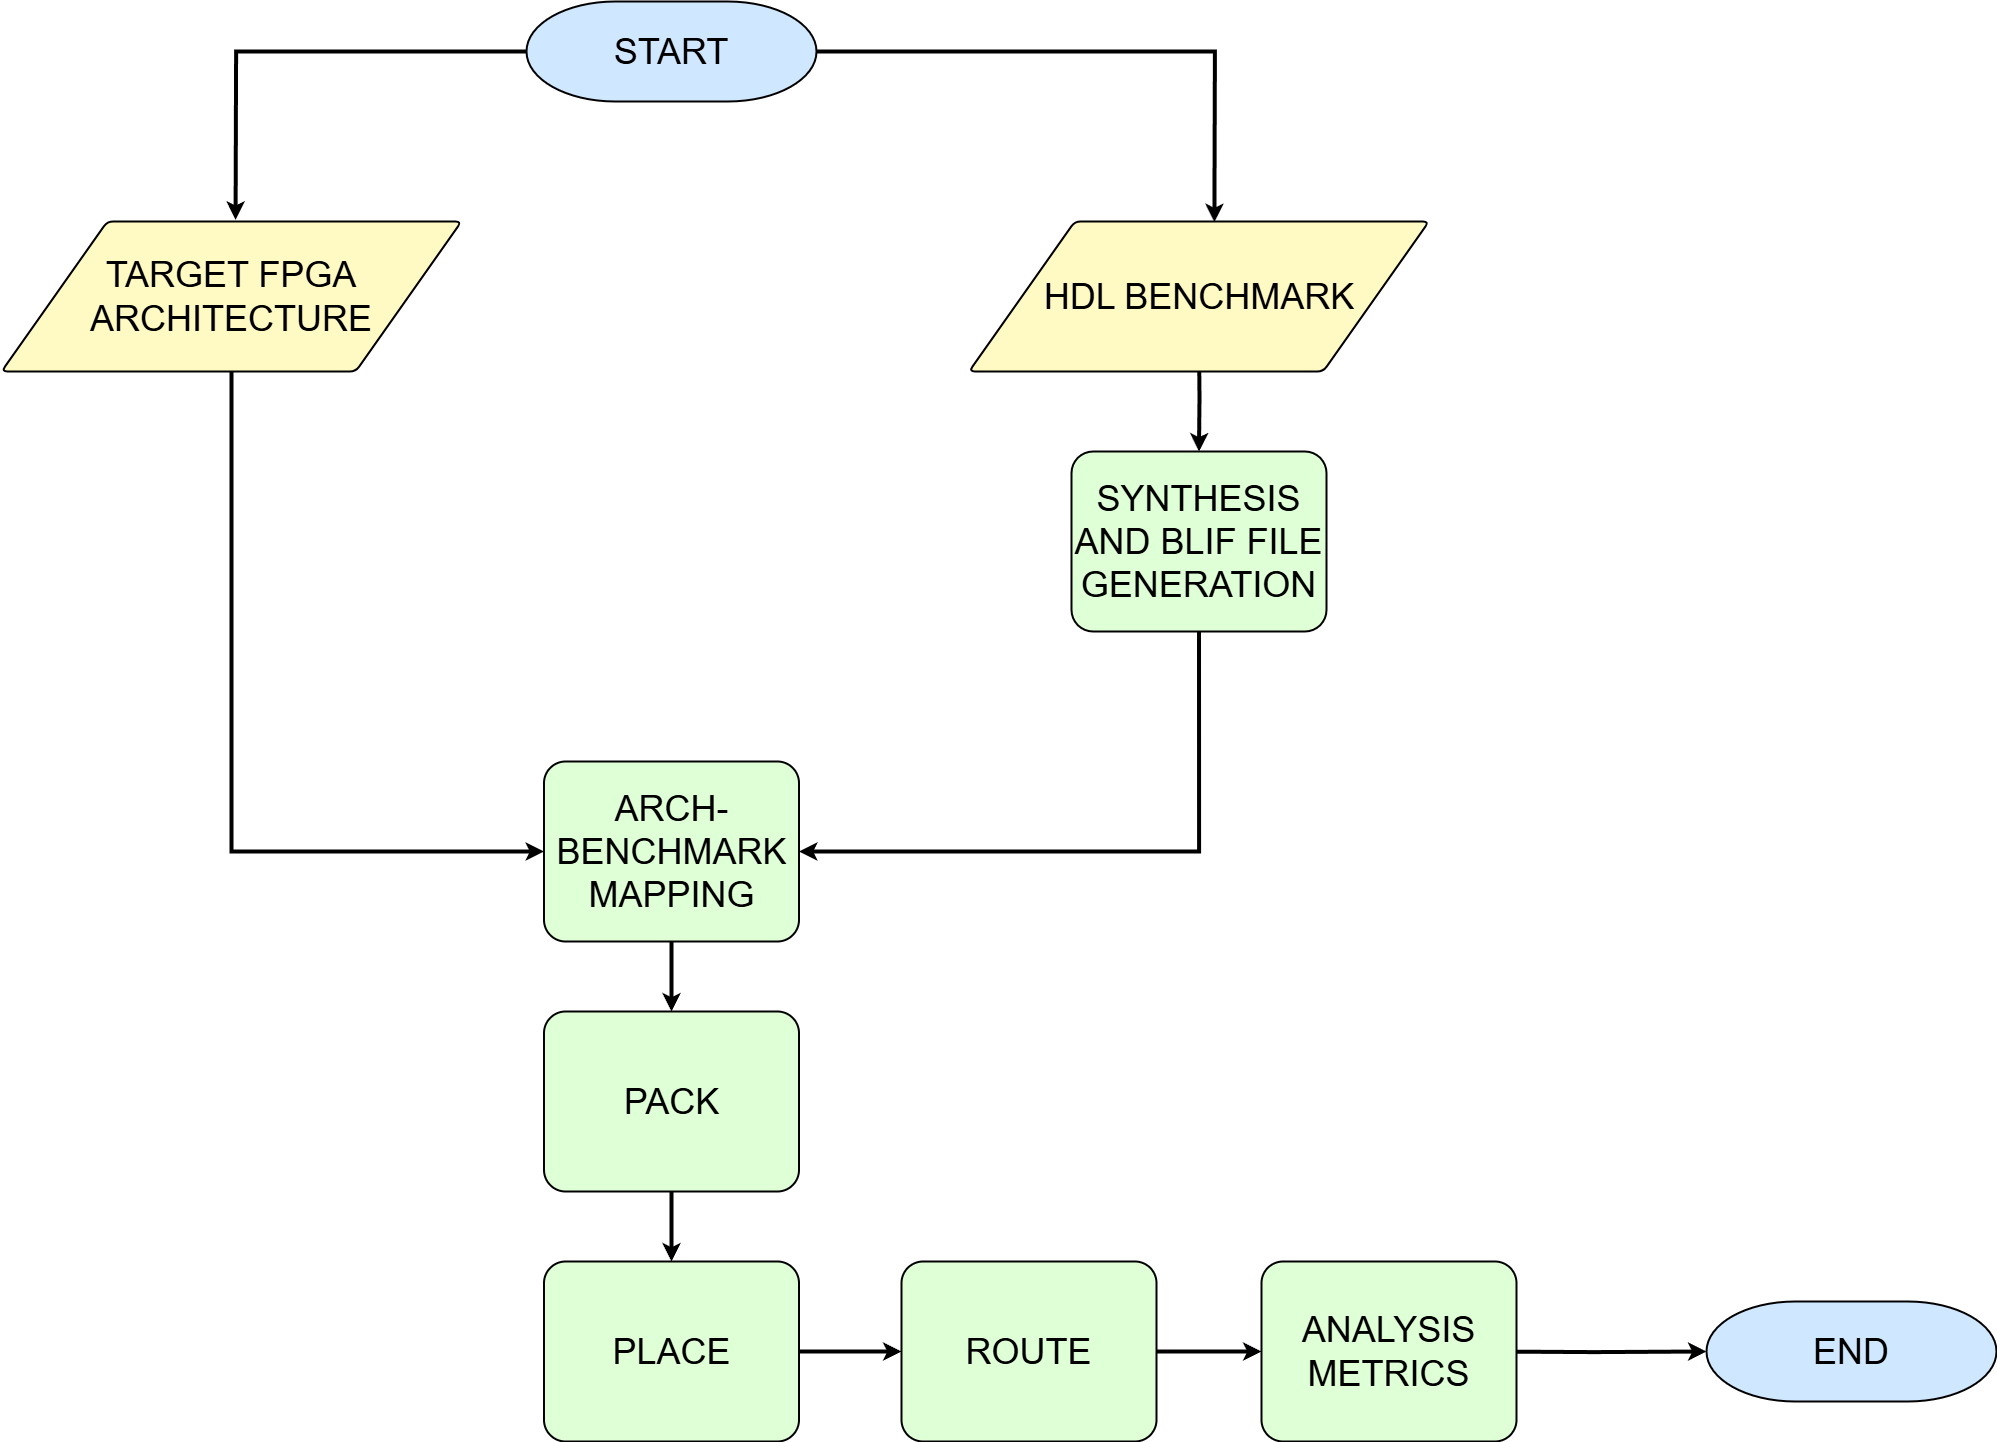
\includegraphics[scale=0.225]{Figures/VTR_Methodology_v2.png}	
	\caption{Methodology of FPGA Architectural Exploration}
	\label{fig:vtr_methodology}
\end{figure}

Parallelly, a domain-specific accelerator named Manojavam is developed using a modular RTL design. It comprises 8 systolic arrays for matrix multiplication, a novel Jacobian Unit for SVD-based eigendecomposition, and a structured cache system. RTL design and simulation are performed using Vivado for FPGA flow, while ASIC design is carried out using the OpenLane toolchain. Floorplanning, timing closure, and power analysis are conducted to validate the feasibility of deployment. The performance of Manojavam is then compared against CPU, GPU, and existing PCA accelerator implementations using a custom-built simulator and various matrix input sizes. The methodology for the design of Manojavam is highlighted in Fig.\ref{fig:manojavam_methodology}.

\begin{figure}[htbp]
	\centering
	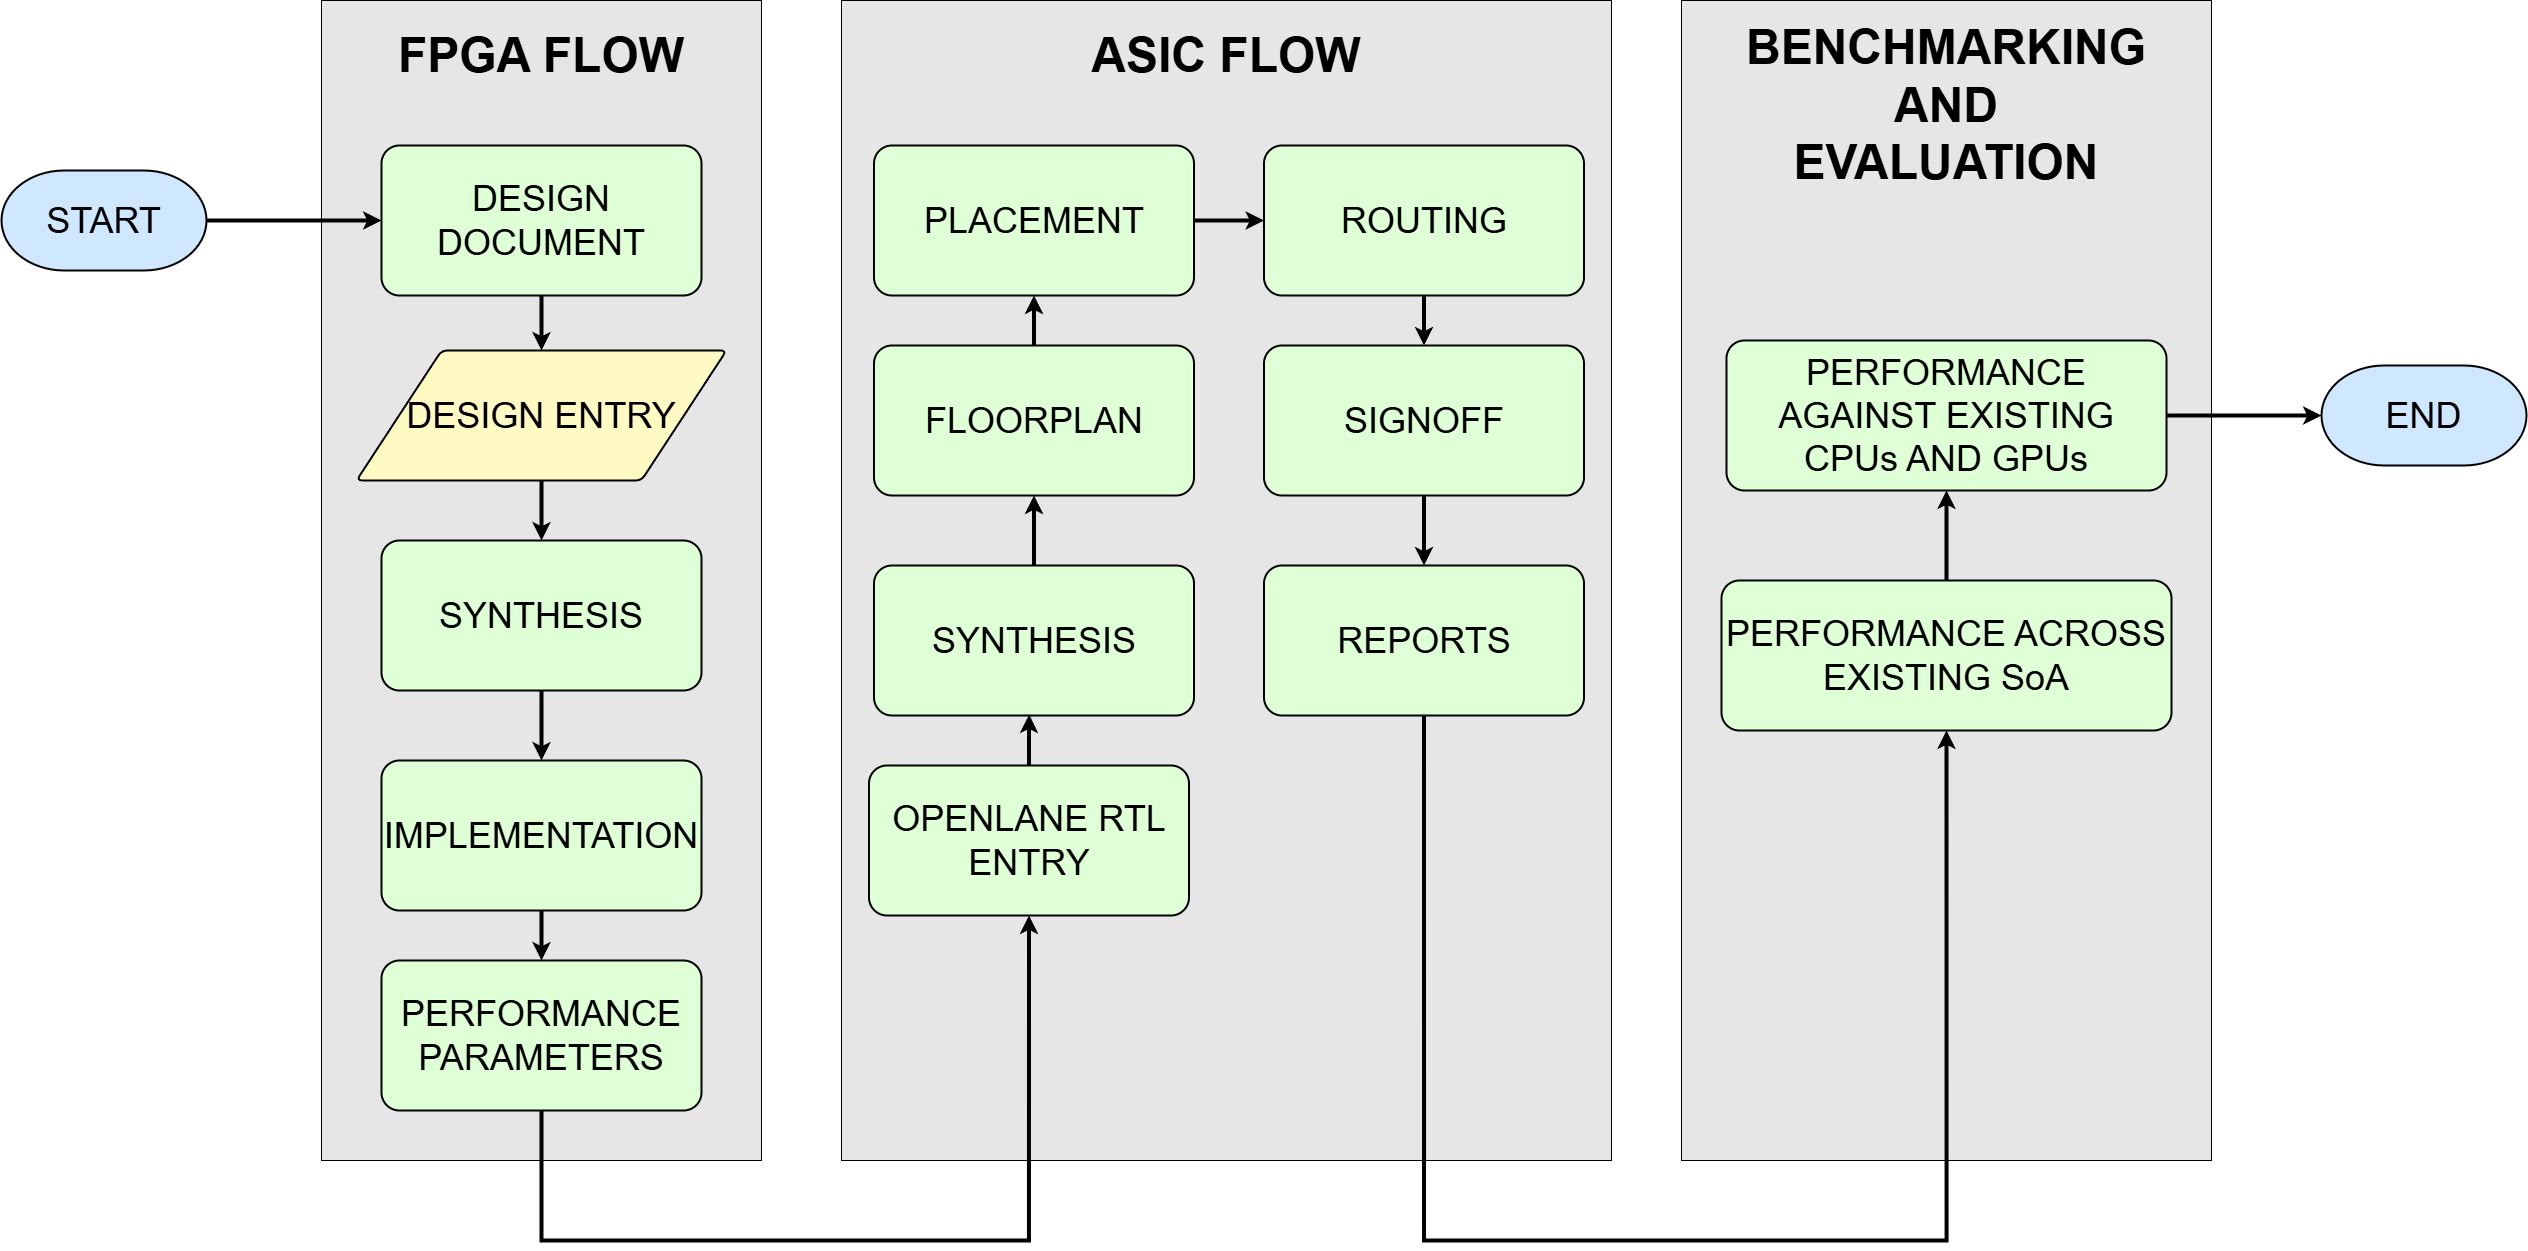
\includegraphics[scale=0.195]{Figures/manojavam_methodology_v2.png}
	\caption{Methodology for Manojavam Accelerator Development}
	\label{fig:manojavam_methodology}
\end{figure}

\begin{comment}
Discuss about the methodology you identified to execute the objectives of your project in brief. Methodology is a system of practices, techniques, procedures, and rules used to execute a particular project. You can elaborate the methodology in a later chapter. Here you can present in the form of a flow diagram and explain the methodology in a paragraph.
\end{comment}

\begin{comment}
\section[Assumptions made / Constraints of the project]{\textbf{Assumptions made / Constraints of the project}}

List the assumptions made for the execution of the project in this section. You can also elaborate on the major constraints of the project. This section should clearly state under what conditions your project is valid. It is mandatory to have this section in your project report.
\end{comment}

\section[Organization of the report]{\textbf{Organization of the report}}

This report is organized as follows. 
\begin{itemize}
\item Chapter 2 discusses the fundamentals and foundational knowledge of FPGA architectures and domain specific acceleration.
\item Chapter 3 discusses the design methodology.
\item Chapter 4 discusses the implementation strategies of both projects.
\item Chapter 5 discusses the results and discussions.
\item Chapter 6 discusses the conclusions and future scope of work.
\end{itemize}

.